\documentclass[11pt]{article}

\usepackage{verbatim}
\usepackage{amsmath}
\usepackage{amssymb}
\usepackage{setspace}
\usepackage[top=1in, bottom=1in, left=1.25in, right=1.25in]{geometry}
\usepackage{subfigure}
\usepackage{graphicx}
\usepackage{cite}
\usepackage[squaren]{SIunits}
\usepackage{listings}

\setlength{\parindent}{0pt} 	% remove the silly paragraph indents

\begin{document}



% ---------------------------------------
% Name section
% ---------------------------------------
\begin{flushleft}
Sherman Lam
\\E155
\\ \today
\end{flushleft}


% ---------------------------------------
% Title
% ---------------------------------------
\begin{center}
\begin{Large}
\textbf{Lab 2 Report: Time-Multiplexed 7-Segment Displays}
\end{Large}
\end{center}


% ---------------------------------------
% Start report
% ---------------------------------------


\section{Introduction}
\label{sec:intro}

In this lab I displayed two 7-segment displays while only using one 7-segment decoder. This is was done by time-multiplexing the two displays. With this technique, one switch is read, decoded, and shown on its corresponding 7-segment display. Then, then the second switch is read, decoded, and shown on its corresponding 7-segment display. Only one 7-segment display is on at a time. The FPGA rapidly switches between the two sets of switches and displays at a rate fast enough to appear steady to the human eye. In addition, the sum of the two switches is displayed on the LED bar on the $\mu$Mudd. \\

Figure \ref{fig:board}, shows the result of the lab. The DIP switches on the breadboard control the left 7-segment display (currently set to 4) and the DIP switches on the $\mu$Mudd control the right 7-segment display (currently set to 2). The sum 6 is displayed on the LED bar using the 5 bottom LEDs. The least significant bit is at the bottom. 

\begin{figure}[h!]
\centering
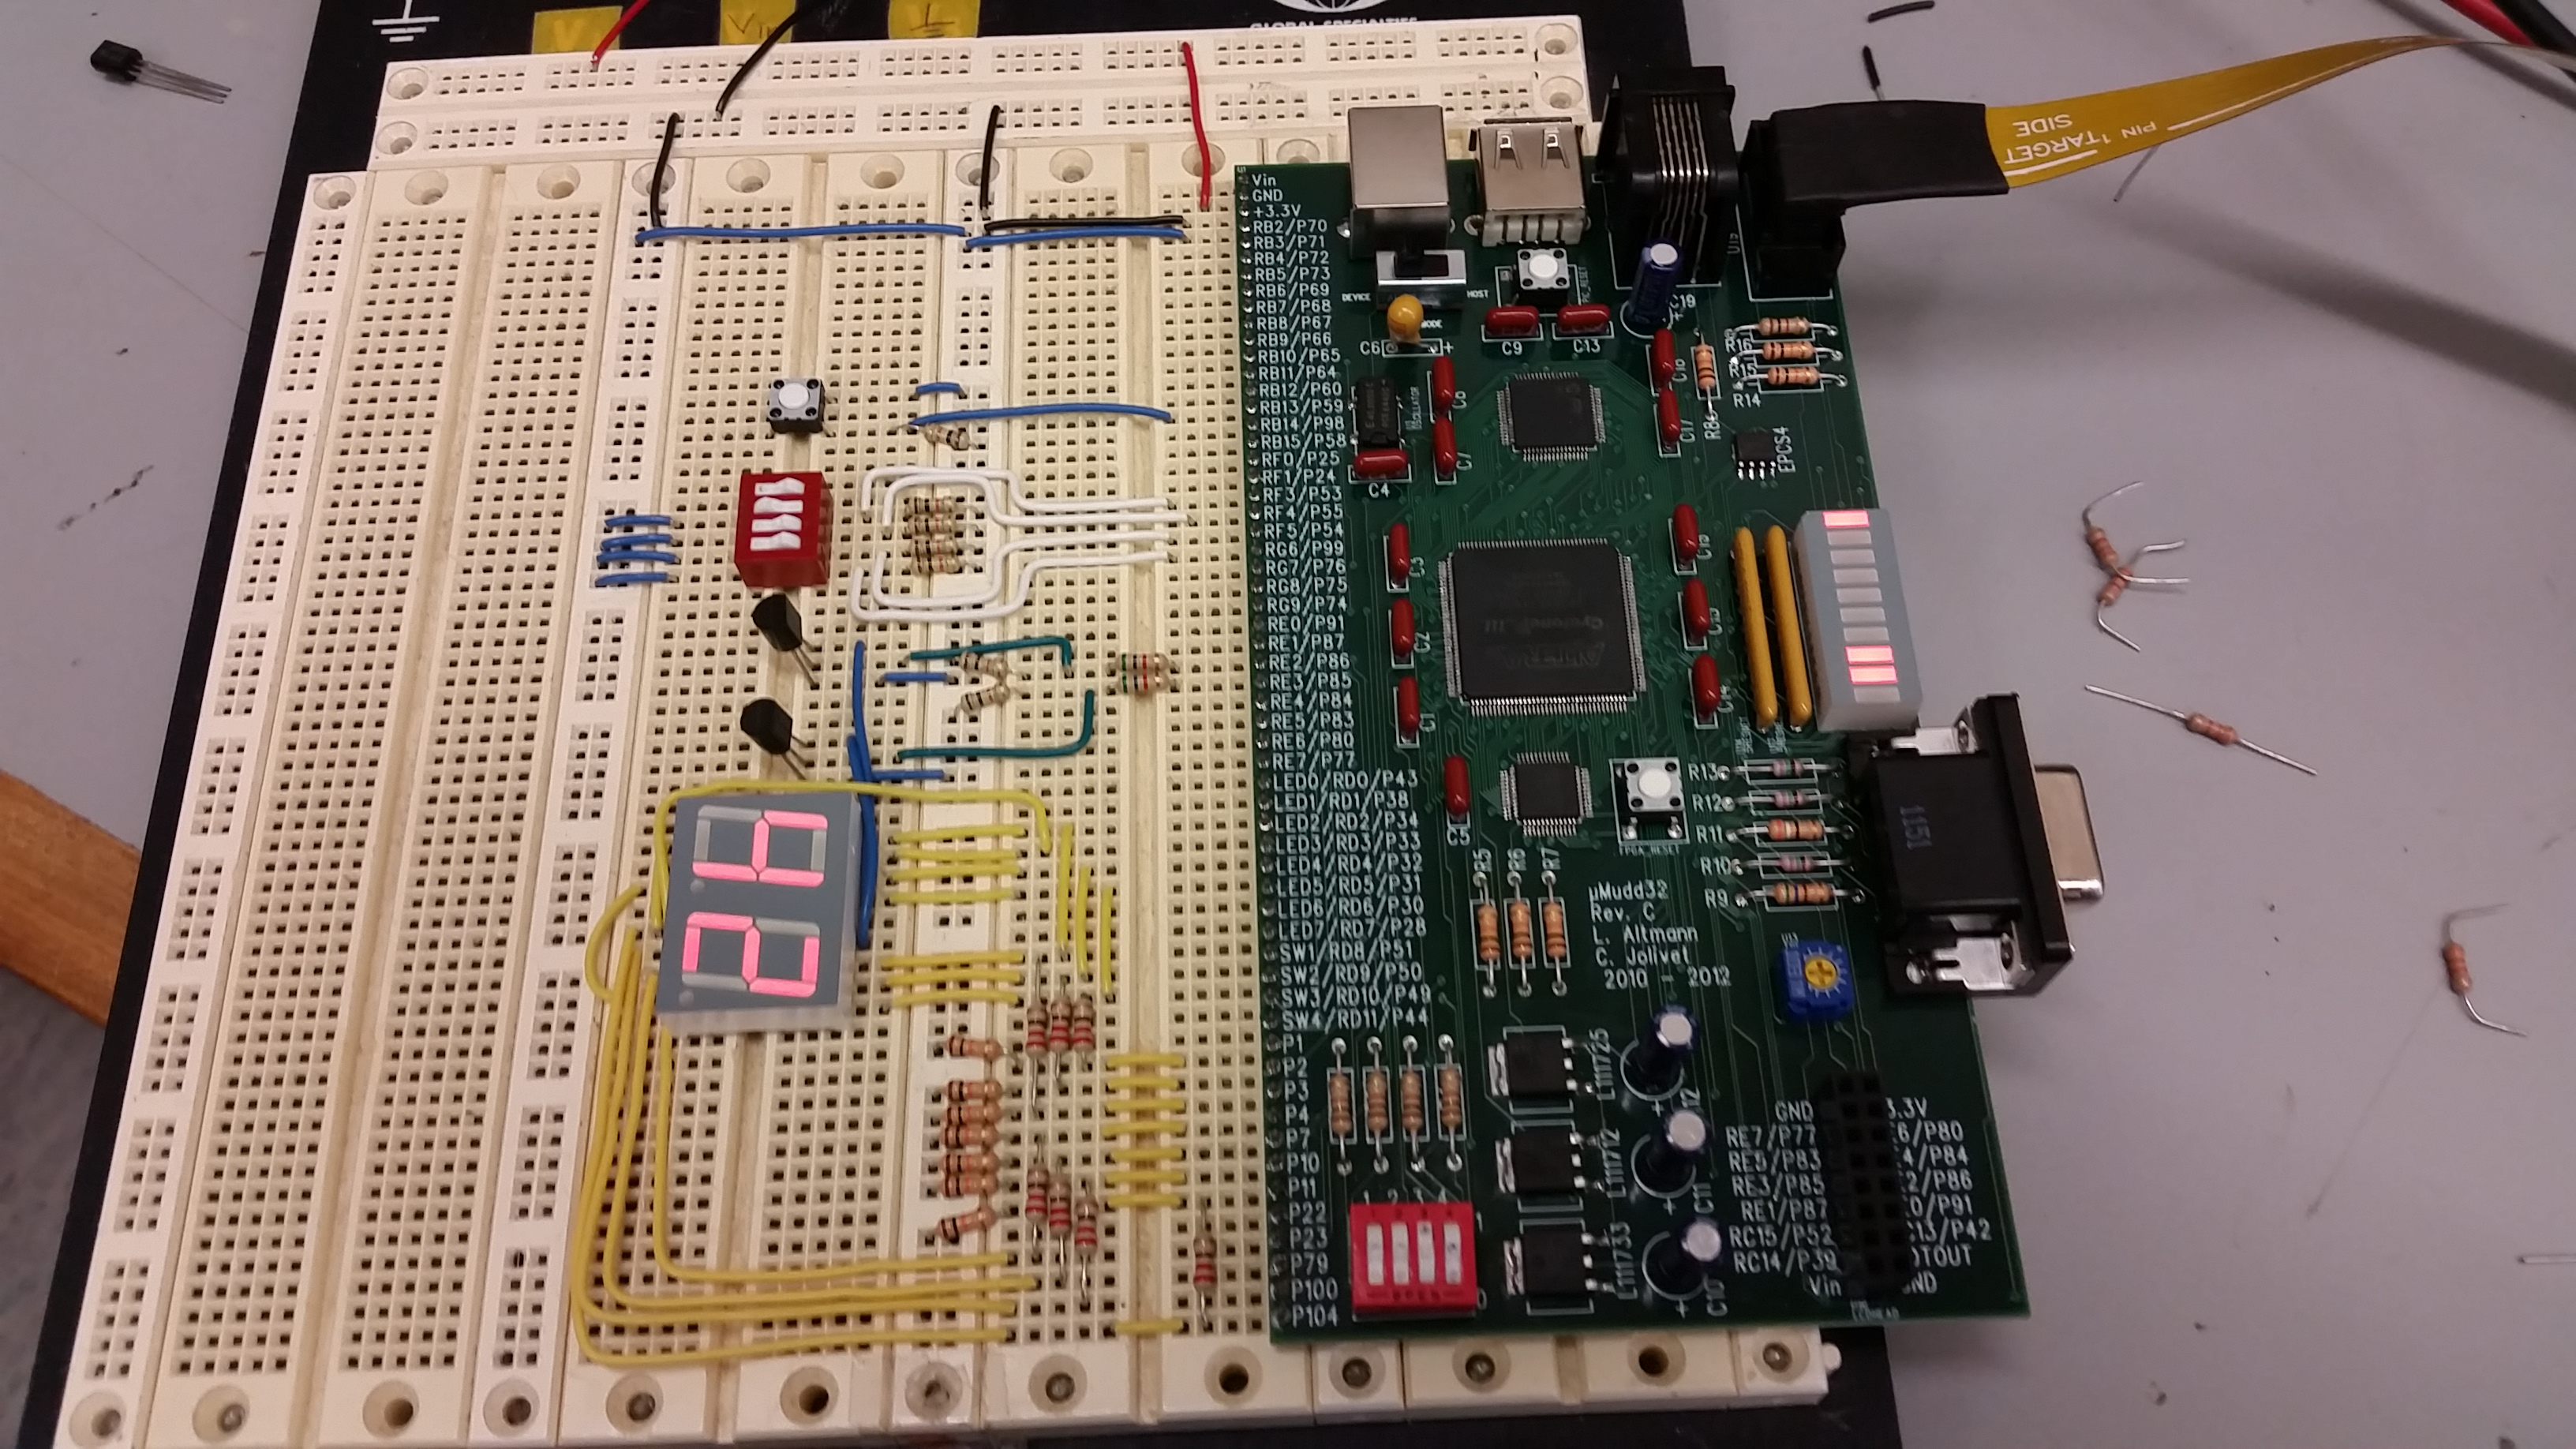
\includegraphics[scale=0.11]{board.jpg}
\caption{Assembled board.}
\label{fig:board}
\end{figure} 


\section{Design and Testing Methodology}


\subsection{Hardware}

A PNP transistor (2N3906) was chosen for toggling the displays because the switch was acting on the anode. The general circuit for using a PNP transistor for switching purposes in shown in Figure \ref{fig:bjt}. If the transistor's based voltage ($V_B$) is brought close to GND, the PNP will turn on. If $V_B$ is brought close to VCC, the transistor will turn off. However, since BJT transistors are current controlled, a resistor ($R_{B}$) must be placed between $V_B$ and its signal pin ($V_{signal}$). To select a value for this resistor, I first considered the largest current draw expected ($I_C$).

\begin{figure}[h!]
\centering
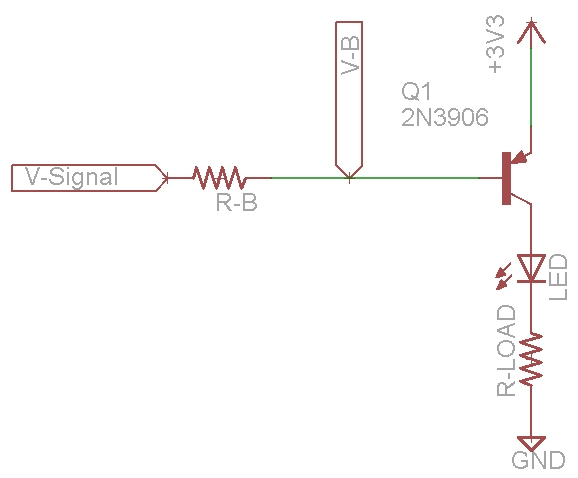
\includegraphics[scale=0.5]{bjt.png}
\caption{General use of a PNP transistor for switching a load}
\label{fig:bjt}
\end{figure} 

\begin{align*}
I_{C} &= (\# segments)*(I_{1segment}) \\
I_{C} &= (\# segments)*(\frac{V_{CC}-V_{led}}{R}) \\
I_{C} &= (\# segments)*(\frac{3.3V-1.7V}{220\Omega}) \\
I_{C} &= 7*(7.3mA) \\
I_{C} &= 51mA
\end{align*}

Then, I considered how much base current ($I_{B}$) I need in order to supply $I_{C}$. The transistor DC current gain (denoted $\beta$ or $h_{FE}$) was approximated from Figure \ref{fig:2N3906_gain} to be 120. So, $I_{B}$ was found to be: 

\begin{align*}
I_{B} &= \frac{I_{C}}{\beta} \\
I_{B} &= \frac{51mA}{120} \\
I_{B} &= 0.4mA
\end{align*}

We can then find the resistor need to supply this voltage when the signal pin is pulled LOW. Because this is a silicon transistor, $V_{EB}=0.7V$.  Note that R was rounded to the nearest resistor value available in the lab. This is okay because the the value of R is not critical. It simply needs to be high enough to prevent the transistor from burning out (if $V_EB$ is too high) and low enough to allow sufficient current to light up the LEDs. If the value of the R is lower than ideal, the transistor will saturate but still function. \\

\begin{align*}
R &= \frac{Vcc-V_{EB}}{I_{B}} \\
R &= \frac{3.3-0.7}{0.4mA} \\
R &= 6.1k\Omega	\\
R &\approx 5.6k\Omega
\end{align*}



\begin{figure}[h!]
\centering
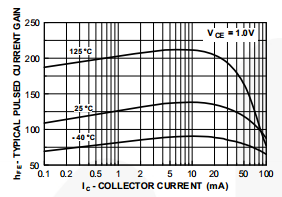
\includegraphics[scale=1]{2N3906_gain.png}
\caption{DC gain of 2N3906 transistor. Image obtained from 2N3906 datasheet.}
\label{fig:2N3906_gain}
\end{figure} 


PNP transistors were also used because MOSFETs were not available. 

\subsection{Software}

Table \ref{table:7seg_decoder} shows how the switch inputs map to the 7-segment outputs. \\


\begin{table}[h]
\centering
\begin{tabular}{|c|c|c|c|c|c|c|c|c|c|c|c|c|}
\hline
\multicolumn{13}{|c|}{7-Segment Display Truth Table}                                  \\ \hline
\multicolumn{5}{|c|}{Inputs}                      & \multicolumn{8}{c|}{Ouputs}       \\ \hline
s{[}3{]} & s{[}2{]} & s{[}1{]} & s{[}0{]} & (hex) & G & F & E & D & C & B & A & (hex) \\ \hline
0        & 0        & 0        & 0        & 0x0   & 1 & 0 & 0 & 0 & 0 & 0 & 0 & 0x40  \\ \hline
0        & 0        & 0        & 1        & 0x1   & 1 & 1 & 1 & 1 & 0 & 0 & 1 & 0x79  \\ \hline
0        & 0        & 1        & 0        & 0x2   & 0 & 1 & 0 & 0 & 1 & 0 & 0 & 0x24  \\ \hline
0        & 0        & 1        & 1        & 0x3   & 0 & 1 & 1 & 0 & 0 & 0 & 0 & 0x30  \\ \hline
0        & 1        & 0        & 0        & 0x4   & 0 & 0 & 1 & 1 & 0 & 0 & 1 & 0x19  \\ \hline
0        & 1        & 0        & 1        & 0x5   & 0 & 0 & 1 & 0 & 0 & 1 & 0 & 0x12  \\ \hline
0        & 1        & 1        & 0        & 0x6   & 0 & 0 & 0 & 0 & 0 & 1 & 0 & 0x02  \\ \hline
0        & 1        & 1        & 1        & 0x7   & 1 & 1 & 1 & 1 & 0 & 0 & 0 & 0x78  \\ \hline
1        & 0        & 0        & 0        & 0x8   & 0 & 0 & 0 & 0 & 0 & 0 & 0 & 0x00  \\ \hline
1        & 0        & 0        & 1        & 0x9   & 0 & 0 & 1 & 1 & 0 & 0 & 0 & 0x18  \\ \hline
1        & 0        & 1        & 0        & 0xA   & 0 & 0 & 0 & 1 & 0 & 0 & 0 & 0x08  \\ \hline
1        & 0        & 1        & 1        & 0xB   & 0 & 0 & 0 & 0 & 0 & 1 & 1 & 0x03  \\ \hline
1        & 1        & 0        & 0        & 0xC   & 0 & 1 & 0 & 0 & 1 & 1 & 1 & 0x27  \\ \hline
1        & 1        & 0        & 1        & 0xD   & 0 & 1 & 0 & 0 & 0 & 0 & 1 & 0x21  \\ \hline
1        & 1        & 1        & 0        & 0xE   & 0 & 0 & 0 & 0 & 1 & 1 & 0 & 0x06  \\ \hline
1        & 1        & 1        & 1        & 0xF   & 0 & 0 & 0 & 1 & 1 & 1 & 0 & 0x0E  \\ \hline
\end{tabular}
\caption{Truth table for 7-Segment LED decoder}
\label{table:7seg_decoder}
\end{table}


Figure \ref{fig:logic} shows the logic flow of the program. on1 is the control signal that decides whether or not the first 7-segment display is on (the first display is set to the left display). Note, because the hardware requires on1 to be pulled LOW in order for the PNP transistor to turn on, s1[3:0] is selected when on1 is 0. Since only one display is on at at time, on2 (the control signal for the second display) is the bitwise NOT of on1. s3 is the value on the selected switch and is passed through the 7-segment decoder to obtain the state of each segment in the display. Even though similar cathodes of both displays share the same state, only the segments in one display will be turned on (as determined by the states of on1 and on2). The sum of both switches are simply passed through an adder to obtain a 5-bit sum. This sum is directly written to the LED bar. See Tables \ref{table:pinmap_ledbar}, \ref{table:pinmap_sevenseg}, \ref{table:pinmap_control}, \ref{table:pinmap_sw1}, and \ref{table:pinmap_sw2} for the pin mappings of each signal. \\


\begin{figure}[h!]
\centering
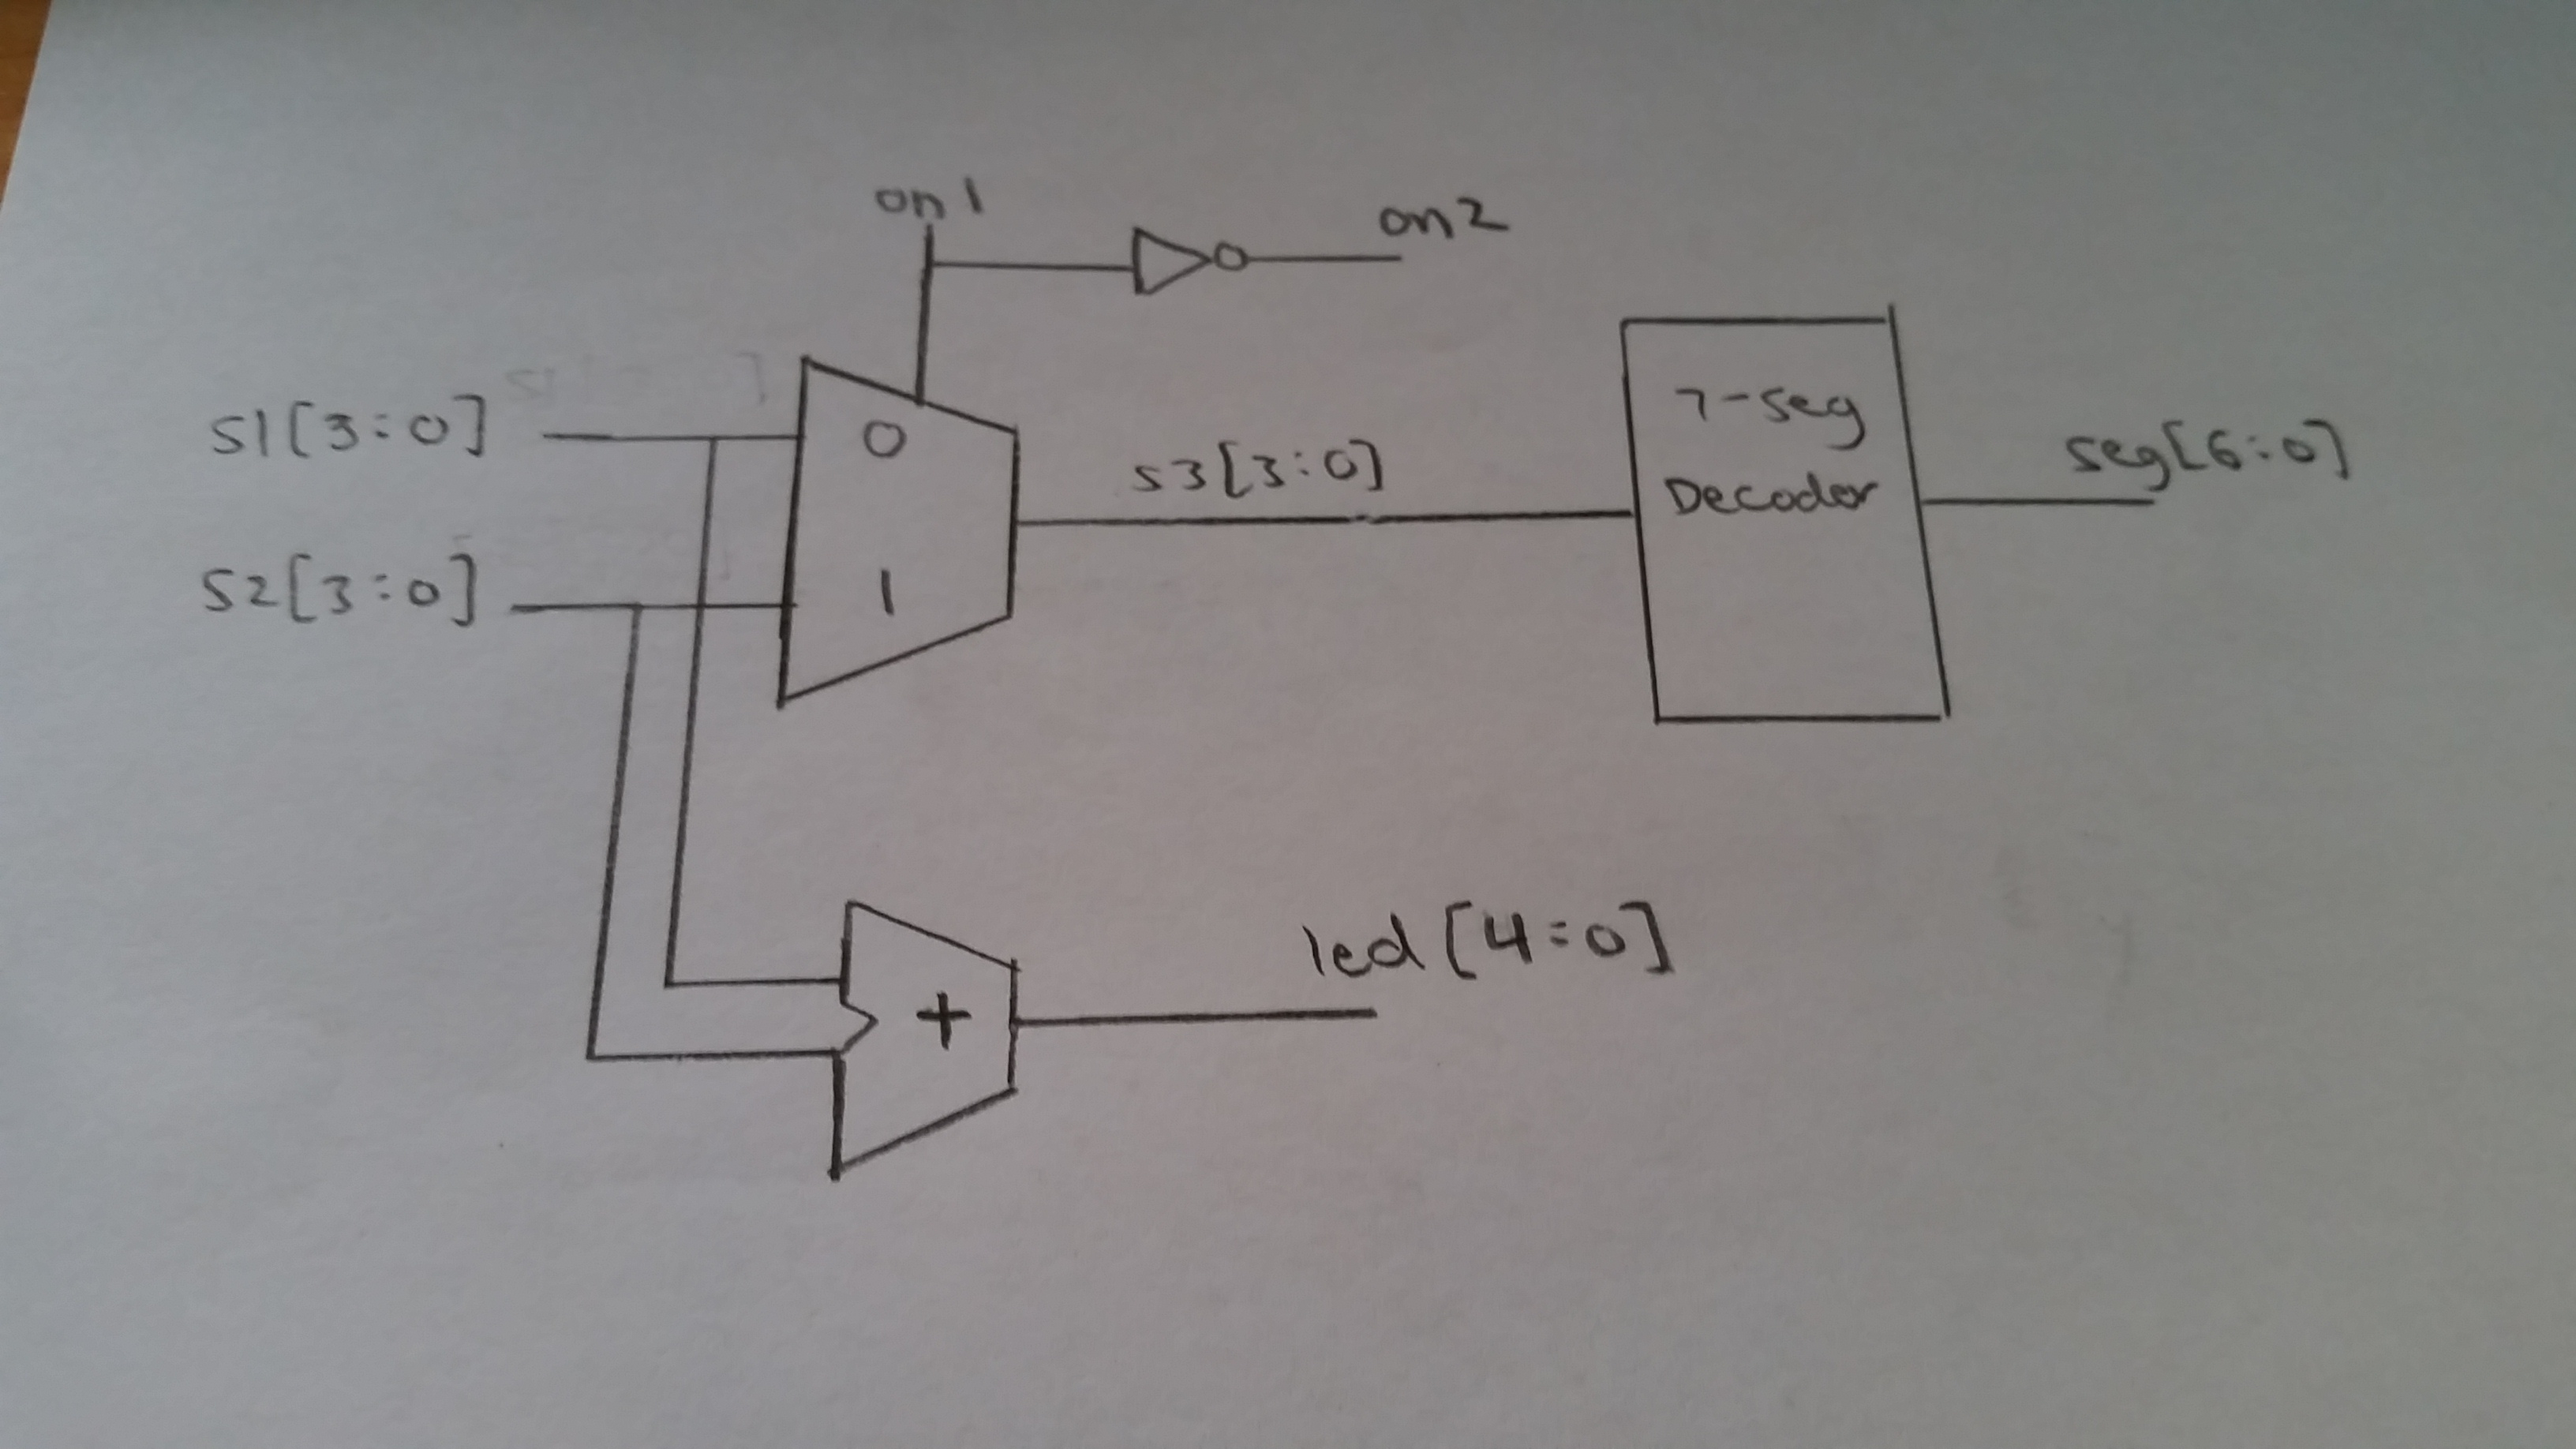
\includegraphics[scale=0.11]{logic.jpg}
\caption{Logic flow of time multiplexer}
\label{fig:logic}
\end{figure} 


\begin{table}[h]
\centering
\begin{tabular}{|c|c|c|c|c|}
\hline
\multicolumn{5}{|c|}{\textbf{LED Bar Pin Mapping}}             \\ \hline
led{[}4{]} & led{[}3{]} & led{[}2{]} & led{[}1{]} & led{[}0{]} \\ \hline
P33        & P32        & P31        & P30        & P28        \\ \hline
\end{tabular}
\caption{Pin mapping of LED bar}
\label{table:pinmap_ledbar}
\end{table}


\begin{table}[h]
\centering
\begin{tabular}{|c|c|c|c|c|c|c|}
\hline
\multicolumn{7}{|c|}{\textbf{7 - Segment Display Pin Mapping}} \\ \hline
seg[0]/A   & seg[1]/B   & seg[3]/C   & seg[4]/D    & seg[5]/E    & seg[6]/F   & seg[7]/G   \\ \hline
P2         & P1         & P4         & P10         & P11         & P3         & P7  \\ \hline
\end{tabular}
\caption{Pin mapping of 7-segment display}
\label{table:pinmap_sevenseg}
\end{table}


\begin{table}[h]
\centering
\begin{tabular}{|c|c|c|c|}
\hline
\multicolumn{4}{|c|}{\textbf{Control Signals Pin Mapping}} \\ \hline
on1        & on2        & clk        & reset       \\ \hline
P87        & P86        & P88        & P60         \\ \hline
\end{tabular}
\caption{Pin mapping of control signals}
\label{table:pinmap_control}
\end{table}


\begin{table}[h]
\centering
\begin{tabular}{|c|c|c|c|}
\hline
\multicolumn{4}{|c|}{\textbf{Switch 1 Pin Mapping}} \\ \hline
s1{[}3{]}  & s1{[}2{]}  & s1{[}1{]} & s1{[}0{]} \\ \hline
P24        & P53        & P55       & P54       \\ \hline
\end{tabular}
\caption{Pin mapping for DIP switch set 1}
\label{table:pinmap_sw1}
\end{table}


\begin{table}[h]
\centering
\begin{tabular}{|c|c|c|c|}
\hline
\multicolumn{4}{|c|}{\textbf{Switch 2 Pin Mapping}} \\ \hline
s2{[}3{]}  & s2{[}2{]}  & s2{[}1{]} & s2{[}0{]} \\ \hline
P51        & P50        & P49       & P44       \\ \hline
\end{tabular}
\caption{Pin mapping for DIP switch set 2}
\label{table:pinmap_sw2}
\end{table}



To flash a display, the display needs to be toggled twice: once to turn on, and once to turn off. Thus, in order for the program to flash the segments at 60Hz, each segment needs to be toggled at 120Hz. The on-board clock oscillates at 40MHz so the LED displays need to be toggled every $\frac{40MHz}{120Hz} \approx 333333$ clock cycles. The 60Hz flashing rate was experimentally determined to be successful at deceiving the human eye.


\label{sec:software_LEDbar}

\clearpage


\subsubsection{Simulation}

The code's logic was tested in ModelSim-Altera. The following show the results of the wave simulations that were run. The program was simulated in sections to ease debugging and wave simulation viewing.

\begin{figure}[h!]
\centering
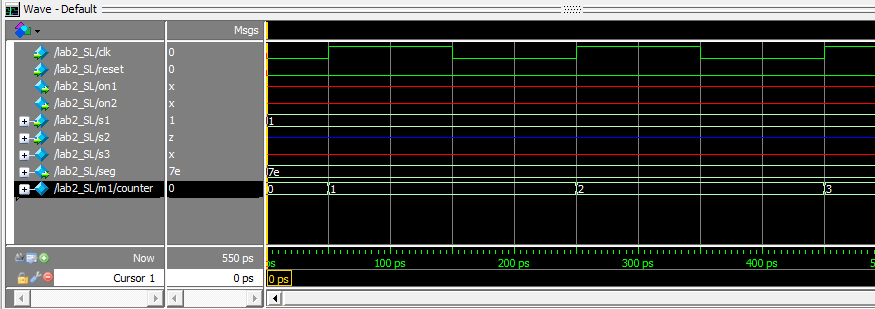
\includegraphics[scale=0.65]{clk_works.png}
\caption{The counter increments at every clock cycle.}
\label{fig:wave_clk}
\end{figure} 


\begin{figure}[h!]
\centering
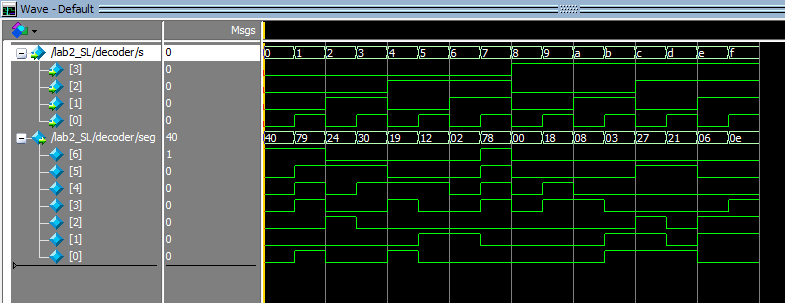
\includegraphics[scale=0.7]{mux_all.png}
\caption{Logic for 7-segment decoder.}
\label{fig:wave_mux}
\end{figure} 


\begin{figure}[h!]
\centering
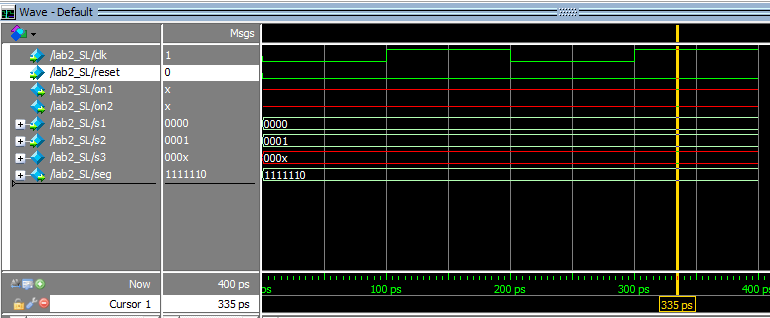
\includegraphics[scale=0.75]{no_reset.png}
\caption{If the reset signal is never HIGH, the control signals for toggling the 7-segment displays (on1 and on2) will not resolve to a logic level.}
\label{fig:wave_reset_no}
\end{figure} 


\begin{figure}[h!]
\centering
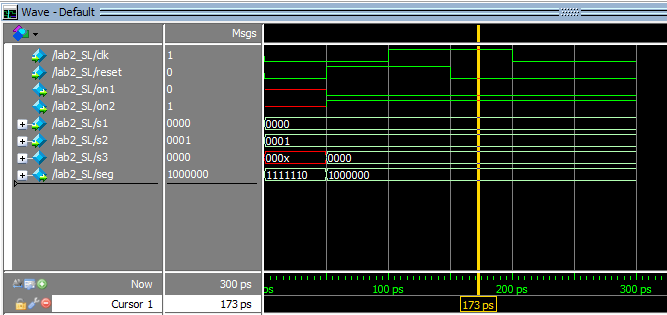
\includegraphics[scale=0.8]{yes_reset.png}
\caption{Once the reset signal is HIGH, the control signals for toggling the 7-segment displays (on1 and on2) are initialized to hard-coded starting values.}
\label{fig:wave_reset_yes}
\end{figure}


\begin{figure}[h!]
\centering
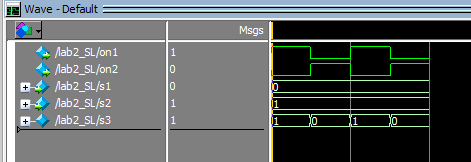
\includegraphics[scale=1]{toggling.png}
\caption{When on1 and on2 will swap states, s3 (the signal used for the 7-segment decoding) changes from s1 to s2 or vice versa.}
\label{fig:wave_toggle}
\end{figure}


\begin{figure}[h!]
\centering
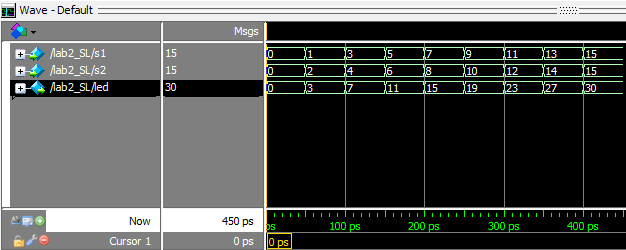
\includegraphics[scale=1]{sum.png}
\caption{The summation of the two input switch values (s1 and s2) is sent to the led bar (led[4:0]).}
\label{fig:wave_sum}
\end{figure}


\clearpage

\section{Technical Documentation}

The following section shows schematics for breadboard circuit that was built. The source code is also provided.

\subsection{7-segment Displays Schematic}

\begin{figure}[h!]
\centering
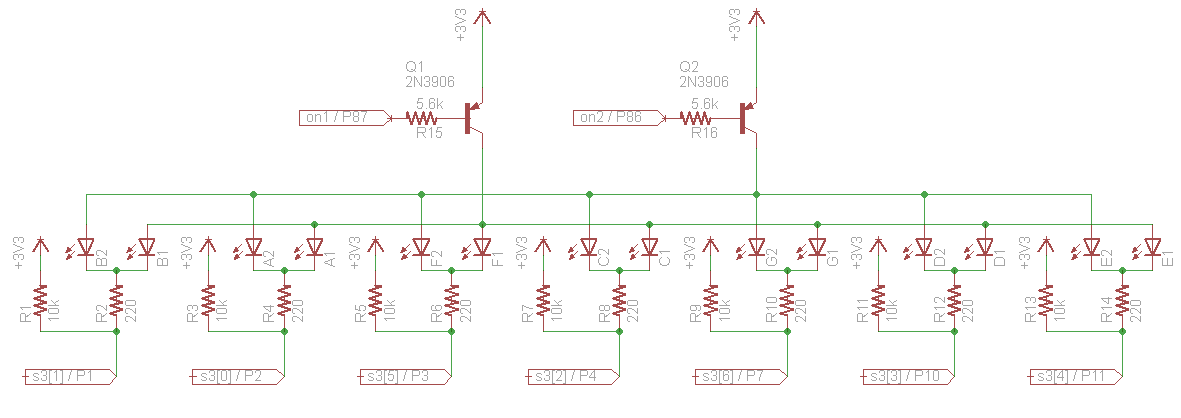
\includegraphics[scale=0.5, angle=90]{seven_segment_all.png}
\caption{Full schematic for dual 7-segment display. Note that on1 and on2 toggle the two displays on and off. Only one or the other is on at any given time.}
\label{fig:seven_seg_sch}
\end{figure} 


\begin{figure}[h!]
\centering
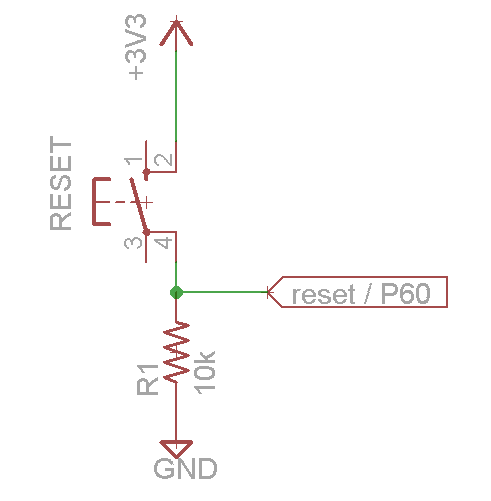
\includegraphics[scale=0.54]{reset.png}
\caption{Schematic for reset button.}
\label{fig:reset_sch}
\end{figure} 


\begin{figure}[h!]
\centering
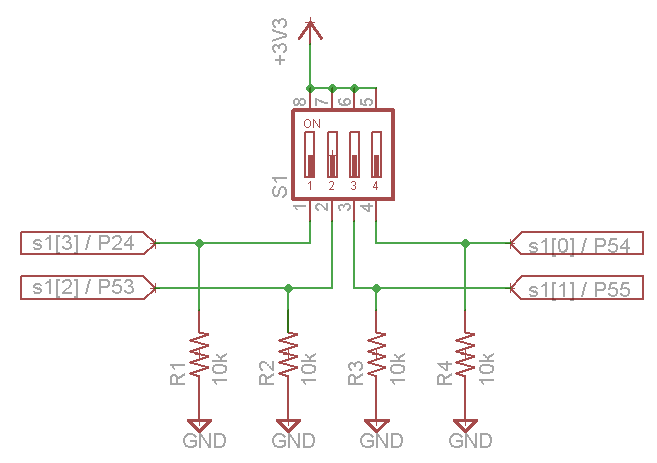
\includegraphics[scale=0.54]{s1.png}
\caption{Schematic for DIP switch 1. This controls display segment 1 (left).}
\label{fig:s1_sch}
\end{figure} 


\begin{figure}[h!]
\centering
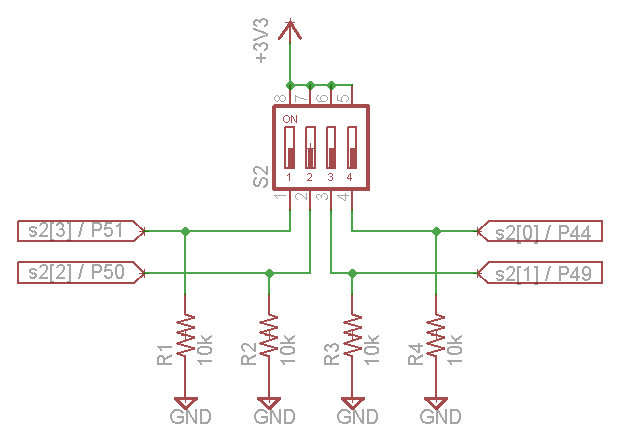
\includegraphics[scale=0.54]{s2.png}
\caption{Schematic for DIP switch 2. This controls display segment 2 (right).}
\label{fig:s2_sch}
\end{figure} 


\clearpage
\subsection{System Verilog Code}

% \small\begin{verbatim}
\begin{lstlisting}[language=Verilog,numbers=left,basicstyle=\footnotesize]

/* This is the main module. It selects which set of switch
   outputs to use and then decodes the number of the selected
   switch. This also sets the clock that time-multiplexes the 
   two 7 segment outputs.
   
   Author: Sherman Lam
   Email: slam@g.hmc.edu
   Date: Sep 17, 2014
*/
module lab2_SL(input logic clk, reset,
               input logic [3:0] s1,s2, //DIP switches
               output logic on1, on2,   //if on1 is pulled LOW, LED set 1 is on.
               output logic [6:0] seg,
               output logic [4:0] led); //segment states    
   
   // time multiplexing
   multiplexer m1(.clk(clk), .on1(on1), .reset(reset));
   
   // the segments always have opposite states.
   assign on2 = ~on1;      
   
   // select the right set of switches.
   // on1 -> s1 is used. on2 -> s2 is used
   // if on1 is pulled LOW, LED set 1 is on.
   logic [3:0] s3;
   assign s3 = on1? s2 : s1;  
   
   // 7 segment decoder
   led7Decoder decoder(.s(s3), .seg(seg));
   
   // sum the outputs and write to LED bar
   assign led = s1 + s2;
   
   
endmodule


/* This module time multiplexes by toggling on1.

   Author: Sherman Lam
   Email: slam@g.hmc.edu
   Date: Sep 17, 2014
*/
module multiplexer(  input logic clk, reset,
                     output logic on1);
   // time multiplexer for switching bewteen displays
   logic [18:0] hPeriod = 19'd333333;  // 120Hz toggling
   logic [18:0] counter = 'b0;
      
   always_ff @(posedge clk, posedge reset) begin
      if (reset)     
         on1 = 1'b0;
      else begin
         if (counter >= hPeriod) begin
            counter = 'b0;
            on1 = ~on1;
         end
         else
            //on1 = on1;
            counter <= counter + 1'b1;
      end
   end
   
endmodule


/* This module decodes the switch inputs into an output for the 
   7 segment display on the development board.
   s[3:0] = [sw3, ... ,sw1]
   seg[6:0] = [g,f, ... ,b,a]
   
   Author: Sherman
   Email: slam@g.hmc.edu
   Date: Sep 9, 2014
*/
module led7Decoder(  input logic [3:0] s,       //4 DIP switches
                     output logic [6:0] seg);   //segments in 7-seg display
                     
   always_comb begin
      //lookup table for s-seg relationship
      case(s)
         4'h0: seg = 7'b100_0000;      // 0x0
         4'h1: seg = 7'b111_1001;      // 0x1
         4'h2: seg = 7'b010_0100;      // 0x2
         4'h3: seg = 7'b011_0000;      // 0x3
         4'h4: seg = 7'b001_1001;      // 0x4
         4'h5: seg = 7'b001_0010;      // 0x5
         4'h6: seg = 7'b000_0010;      // 0x6
         4'h7: seg = 7'b111_1000;      // 0x7
         4'h8: seg = 7'b000_0000;      // 0x8
         4'h9: seg = 7'b001_1000;      // 0x9
         4'ha: seg = 7'b000_1000;      // 0xA
         4'hb: seg = 7'b000_0011;      // 0xB
         4'hc: seg = 7'b010_0111;      // 0xC
         4'hd: seg = 7'b010_0001;      // 0xD
         4'he: seg = 7'b000_0110;      // 0xE
         4'hf: seg = 7'b000_1110;      // 0xF
         default: seg = 7'b111_1110;      // default to a dash
      endcase
      
   end
endmodule



\end{lstlisting}
% \end{verbatim}


\clearpage

\section{Results and Discussion}

The system works as expected. The number set by the DIP switches on the breadboard is displayed on the left 7-segment display. The number set by the DIP switches on the $\mu$Mudd is displayed on the right 7-segment display. The FPGA flashes both displays at 60Hz. This flashing is unnoticeable when viewed by the human eye. Since each display is operating at 50$\%$ duty cycle, the intensity of the display is about half that of a display being held on (100$\%$ duty cycle). In addition, when the reset button is pressed, display 1 (left) turns on and display 2 (right) turns off. This states is held until the reset button is released. The sum of the values on the two switches is correctly displayed on the LED bar. \\


\section{Conclusion}

\subsection{Time Spent}

\begin{description}
	\item[Programming, Simulating] 2.5hrs
	\item[Breadboarding] 2hrs
	\item[Writing Report] 5hrs
	\item[Total Time Spent] 9.5hrs
\end{description}

\subsection{Suggestions for lab}

The current lab asks the student to use the DIP switches on the $\mu$Mudd in addition to 4 wires to control the two 7-segment displays. However, many people were asking if 4 wires meant an extra set of DIP switch. The instructions seem confusing in regards to this detail. Unless the lab's goal is to purposefully give semi-ambiguous instructions in order to force students to think (channeling E80, eh?), I would suggest explicitly give instructions to use a second set of DIP switches. \\

Also, using MOSFETs may making the switching much easier. Maybe you could consider stocking the E155 Lab with some?


\end{document}

